\section{النموذج المقترح\label{section:my_model}}
كما ذكرنا فإن معظم الملاحقات الحديثة تستخدم المعلومات المكانية فقط أي  معلومات مظهر الهدف. كما في 
\textLR{SwinTrack\cite{swinTrack}}
 وغيرها. 
لكن كان هناك بعض المحاولات للاستفادة من المعلومات الزمانية كما في  خوارزمية
\textLR{STARK\cite{Stark}}،
وذلك من خلال إدخال صورة الغرض الجديد الناتج عن الملاحقة كدخل ثالث، كما هو مذكور في الفقرة 
\ref{section:stark}.
\newline
أما في خوارزمية
\textLR{SwinTrack}
والتي هي النموذج الأساسي في بحثنا، فإنها تعتمد فقط على الـ
\textLR{template}
المأخوذ من أول إطار في الملاحقة كدخل أول، ونافذة البحث كدخل ثاني، أي أن التغيرات التي تطرأ على الغرض لا يتم أخذها بعين الاعتبار.
\newline
الفكرة الأساسية من البحث هي الاستفادة من المعلومات الزمانية، كما في ملاحق 
\textLR{STARK\cite{Stark}}،
لتعديل نموذج
\textLR{SwinTrack\cite{swinTrack}}،
وذلك بأخذ صورة الغرض الناتجة عن الملاحقة
و سنسميها
\textLR{dynamic template}
أو الـ
\textLR{template}
الجديد
كدخل ثالث للخوارزمية.
\newline
وكما هو موضح في المخطط 
\ref{fig:my_model}
والذي يوضح التعديل الذي قمنا به على خوارزمية 
\textLR{SwinTrack\cite{swinTrack}}،
 فإن خوارزميتنا تستخرج سمات الـ
\textLR{template}
الجديد
عبر 
\textLR{Swin backbone}،
فيصبح لدينا سمات الـ
\textLR{template}
الابتدائي و سمات الـ
\textLR{template}
الجديد
بحاجة إلى دمج ومعالجة.
\newline 
كان لدينا عدة خيارات لدمج سمات الـ
\textLR{template}
الجديد:
\begin{itemize}
\item
الخيار الأول كما في ملاحق
\textLR{STARK}
وملاحق
\textLR{SwinTrack}
بأن يتم الدمج عن طريق سَلسَلة
\textLR{concatenate} 
سمات الثلاث مداخل في سلسلة واحدة، ونستخدمها كدخل للمرمز لتدريبه على كشف المعلومات الزمانية والمكانية معاً.
\newline
يتطلب هذا الخيار تعديل في عدد أوزان الترميز المكاني 
\textLR{PE}، 
وبالتالي سنضطر لتدريب هذه الأوزان الجديدة مع تدريب كامل النموذج والتي عددها $23$ مليون وزن من أجل نموذج 
\textLR{SwinTrack-T}
\textLR{\cite{swinTrack}}.
وهذا قد يستغرق أكثر من شهر باستخدام وحدة معالجة الرسومات 
\textLR{GPU}
المتوفرة لدينا وهي 
\textLR{NVIDIA GeForce 2080 Ti}،
ومن أجل 
\textLR{epoches = 300}
كما في تدريب النموذج الأصلي على مجموعة معطيات 
\textLR{Got10k\cite{got10k}}.
لذلك وجب التفكير بطريقة ثانية نستفيد من خلالها من أوزان النموذج الأصلي المدرب مسبقاً.
\item 
الخيار الثاني هو دمج وتعديل سمات الـ
\textLR{template}
الابتدائي مع سمات الـ
\textLR{template}
الجديد بطريقة تحافظ على أبعاد دخل المرمز.
\newline
الطريقة المقترحة هنا هي بتطبيق التابع الأساسي في المحول، وهو تابع الانتباه المشروح بشكل مفصل في الفقرة
\ref{section:attention}.
يضمن لنا تابع الانتباه المحافظة على الأبعاد من جهة، ومن جهة أخرى فإن مصفوفات 
$W_K,W_Q,W_V$
يتم تدريبها لتتعلم دمج السمات.
باستخدام هذا التابع تجنبنا تدريب النموذج بالكامل، وركزنا فقط على تدريب تابع الانتباه
\end{itemize}
باختيارنا للخيار الثاني استخدمنا تابع الانتباه التقاطعي باختيار سمات الـ
\textLR{template}
المعدل كـ
\textLR{query}،
واختيار سمات الـ 
\textLR{template}
الابتدائي كـ
\textLR{key}
و
\textLR{value}، 
فيكون دخل المرمز بحسب المعادلات 
\textLR{\ref{eq:MHA}}
\begin{equation}
\begin{split}
&\text{\textLR{MultiHead}}(Q, K, V) = \text{\textLR{Concat}}(head_1,\dots,head_h)W^O\\
&head_i = \text{\textLR{Attention}}(QW_i^Q, KW_i^K, VW_i^V)\\
\end{split}
\label{eq:MHA}
\end{equation}
\newline
حيث 
$i$
هو رقم الرأس في كتلة الانتباه التقاطعي متعدد الرؤوس.
يوضح الشكل 
\ref{fig:my_model}
 التعديل الذي أجريناه في خوارزمية
\textLR{swinTrack}
لدمج المعلومات الزمانية والمكانية.
يتم تعديل الـ
\textLR{ updated template}
بحسب خرج شبكة التصنيف والتي تعبر عن
\textLR{  IOU }
المتنبأ به.
 نختار الـ
 \textLR{template}
 الجديد إذا تحقق
\textRL{شرطان}
 معاً وهما:
 \begin{itemize}
 	\item
 	خرج شبكة التصنيف 
 	%\textLR{IOU-aware classification}
 	أكبر من حد معين
 	\textLR{IOU threshold}
 	\item
 	عدد الإطارات بعد آخر تحديث
	\textLR{update interval}
 	 أكبر من قيمة معينة 
 	وذلك كما في خوارزمية 
 	\textLR{STARK\cite{Stark}}.
 \end{itemize}

\subsection{التدريب}
بما أن النموذج المقترح يستخدم شبكتي تصنيف و
\textLR{regression}
فإنه يحتاج إلى تابعي خطأ مستقلين من أجل عملية التدريب، سنذكر كل منهما في هذه الفقرة.
\subsubsection{تدريب التصنيف}
نستخدم من أجل عملية تدريب شبكة التصنيف تابع الخطأ 
\textLR{varifocal loss\cite{varifocal}}
مع 
\textLR{IOU-aware classification score}،
هذا التابع يستبدل القيمة
$1$ 
من أجل العينات الموجبة (هدف)، والقيمة 
$0$
للعينات السلبية ( خلفية)، بقيمة
\textLR{IOU}
بين المستطيل المحيط المتنبأ به وبين القيمة الحقيقة
\textLR{ground truth}
لمعطيات التدريب
وذلك أثناء عملية التدريب
\textLR{\cite{generalfocalloss},\cite{varifocal}}،
كما توضحه المعادلات 
\ref{eq:vlclass}،
\ref{eq:vlregress}.
\newline
هذا المعيار يدمج تدريب قيمة الـ
\textLR{IOU}
مع تدريب التصنيف، وهو قادر على مساعدة النموذج بالتنبؤ بالمستطيل المحيط بدقة أكبر.
\begin{equation}
VFL(p,q) = \begin{cases}
-q(q\log(p) + (1-q)\log(1-p)) &  q > 0 \\
-\alpha p^\gamma \log(1-p) &  q=0 \\
\end{cases}\\
\label{eq:vlclass}
\end{equation}

\begin{equation} 
\mathbb{L}_{cls} = VFL(p,IOU(b,\hat{b}))
\label{eq:vlregress}
\end{equation}

حيث
$q$ 
هي قيمة
\textLR{IOU}
، و
$p$
هي خرج شبكة التصنيف تعبر عن احتمالية وجود الغرض، 
$b$:
المستطيل المحيط المتنبأ به،
$\hat{b}$:
المستطيل المحيط الحقيقي في معطيات التدريب
\textLR{ground truth}.
\newline
\subsubsection{تدريب الـ
\textLR{regression}}
من أجل تدريب شبكة الـ
\textLR{regression}
نستخدم تابع الخطأ
\textLR{Generalized IOU\cite{giou}}
بحسب المعادلة
\textLR{\ref{eq:giou}}
\begin{equation} 
\mathbb{L}_{reg} =\sum_{j} \mathds{1}_{q > 0} [p\mathbb{L}_{GIOU}(b_j,\hat{b})]
\label{eq:giou}
\end{equation}
وذلك فقط من أجل
$IOU=q>0$،
أي يتم تجاهل العينات السلبية التي تمثل الخلفية أثناء التدريب، ويتم إعطاء أهمية أكبر للعينات ذات الاحتمالية العالية
وذلك بتوزين تابع الخطأ 
\textLR{GIOU}.
\newline
وكما في خوارزمية 
\textLR{STARK}
فإنه يتم استخدام تابع خطأ مكون من مجموع موزن لتابعي الخطأ السابقين لتدريب النموذج الكلي.
يتم تحديد أوزان النموذج باستخدام خوارزمية الأمثلة
\textLR{AdamW\cite{AdamW}}.
\begin{figure}[!h]
	\centerline{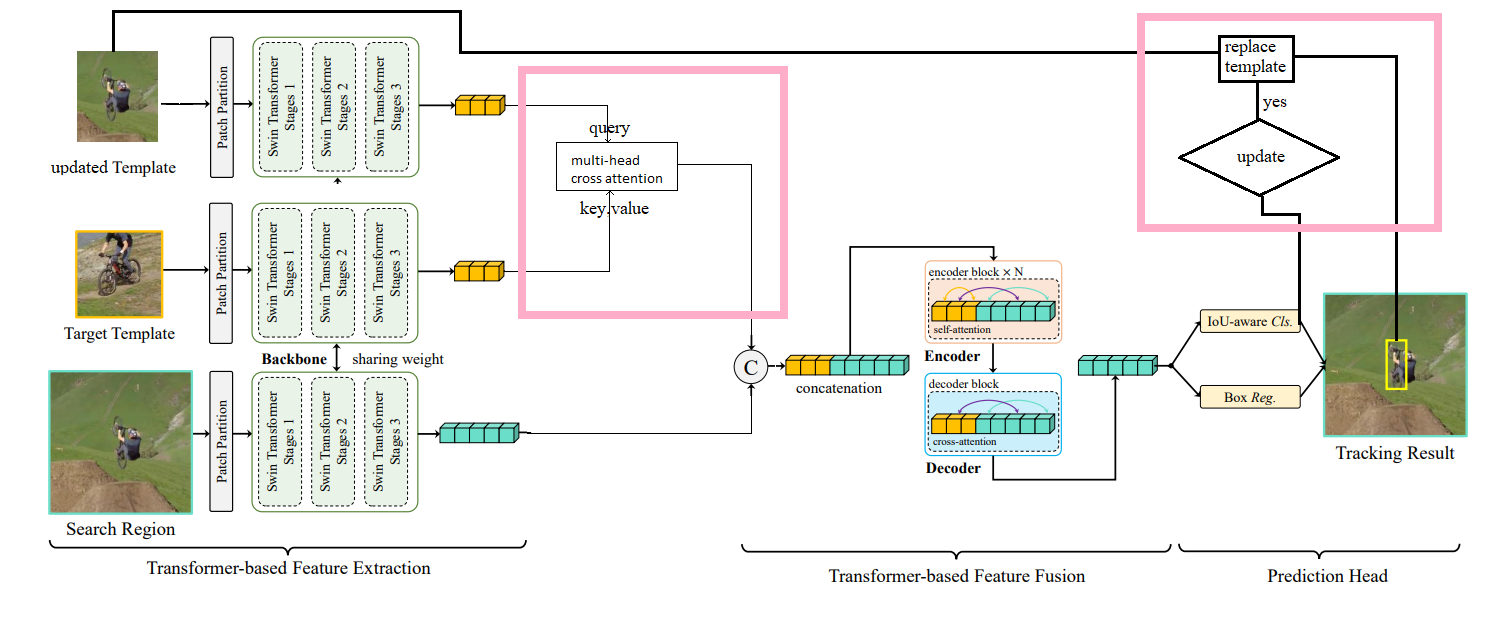
\includegraphics[width=\textwidth]{images/my_model}}
	\caption{\textRL{بنية النموذج المقترح والذي يقوم بدمج سمات صورتي الغرض عبر كتلة انتباه}}
	\label{fig:my_model}
\end{figure}
\section{خاتمة}
تحدثنا في هذا الفصل عن النموذج الأساسي في بحثنا وهو
\textLR{swinTrack}،
وبينا أن مشكلته اعتماده فقط على المعلومات المكانية، بالرغم من سرعته وتفوقه في الأداء على كثير من الملاحقات.   اعتمدنا عندها على طريقة خوارزمية
\textLR{STARK}
في إدخال المعلومات الزمانية. لذلك اقترحنا نموذج يستفيد من معلومات تغير المظهر كمعلومات زمانية، دون تغيير في بنية النموذج الأصلي، للاستفادة من أوزانه في عملية التدريب. وبما أن هذا التعديل قد حسن من أداء 
\textLR{STARK}
فقد توقعنا في بداية مرحلة البحث أنه سيحسن أداء 
\textLR{SwinTrack}.
